\documentclass{jsarticle}
\oddsidemargin=-0.8cm
\topmargin=-2cm
\baselineskip=13pt
\textheight=55\baselineskip
\marginparsep=0.5in
\marginparwidth=0.5in
\textwidth=52zw
\usepackage{ascmac}
\usepackage{url}
\usepackage[dvips]{graphicx}
\usepackage{amsmath}
\usepackage{amssymb}
\usepackage{multicol}
\usepackage{bm}
\usepackage{enumerate}
\usepackage{listings}
\usepackage{fancybox}
\usepackage{framed}
\usepackage{subfigure}
\usepackage{ccaption}
\usepackage{color}
\makeatletter
\lstset{% 
language={C}, 
frame=trbl,% 
basicstyle={\small},% 
identifierstyle={\small},% 
commentstyle={\small\ttfamily},% 
keywordstyle={\small\bfseries},% 
ndkeywordstyle={\small},% 
stringstyle={\small\ttfamily}, 
tabsize=2,
breaklines=true, 
frame=none,
columns=[l]{fullflexible},% 
numbers=left,% 
xrightmargin=0zw,% 
xleftmargin=3zw,% 
numberstyle={\scriptsize},% 
stepnumber=1, 
numbersep=1zw,% 
backgroundcolor={\color[gray]{.90}},
} 
\makeatother

\newenvironment{problems}
{
  \renewcommand\labelenumi{\doublebox{\arabic{enumi}}}
  \begin{enumerate}
}{
  \end{enumerate}
  \renewcommand\labelenumi{\arabic{enumi}.}
}

\pagestyle{empty}	

\begin{document}
\title{基礎気象学講義 復習問題} % ここは毎回同じ
\author{第12回} %authorの代わりに第何回かを入れる
\date{メソ気象学 後編:局地風} %内容を記載する
\maketitle

\section{問題}

    \begin{problems}
    \item 次の問いに答えなさい。
        \begin{enumerate}[(1)]
        \item 海陸風・山谷風について、その周辺の大気の流れを示す図を描きなさい。
        \item 斜面を下る冷気塊は斜面に沿うか離れるか、どちらか答えなさい。根拠も示すこと。\\
        \end{enumerate}

    \item 図\ref{CloudAtlas}に示すのは、5型(CM=5)の中層雲と呼ばれる高積雲である。
        \begin{figure}[h]
        \centering
        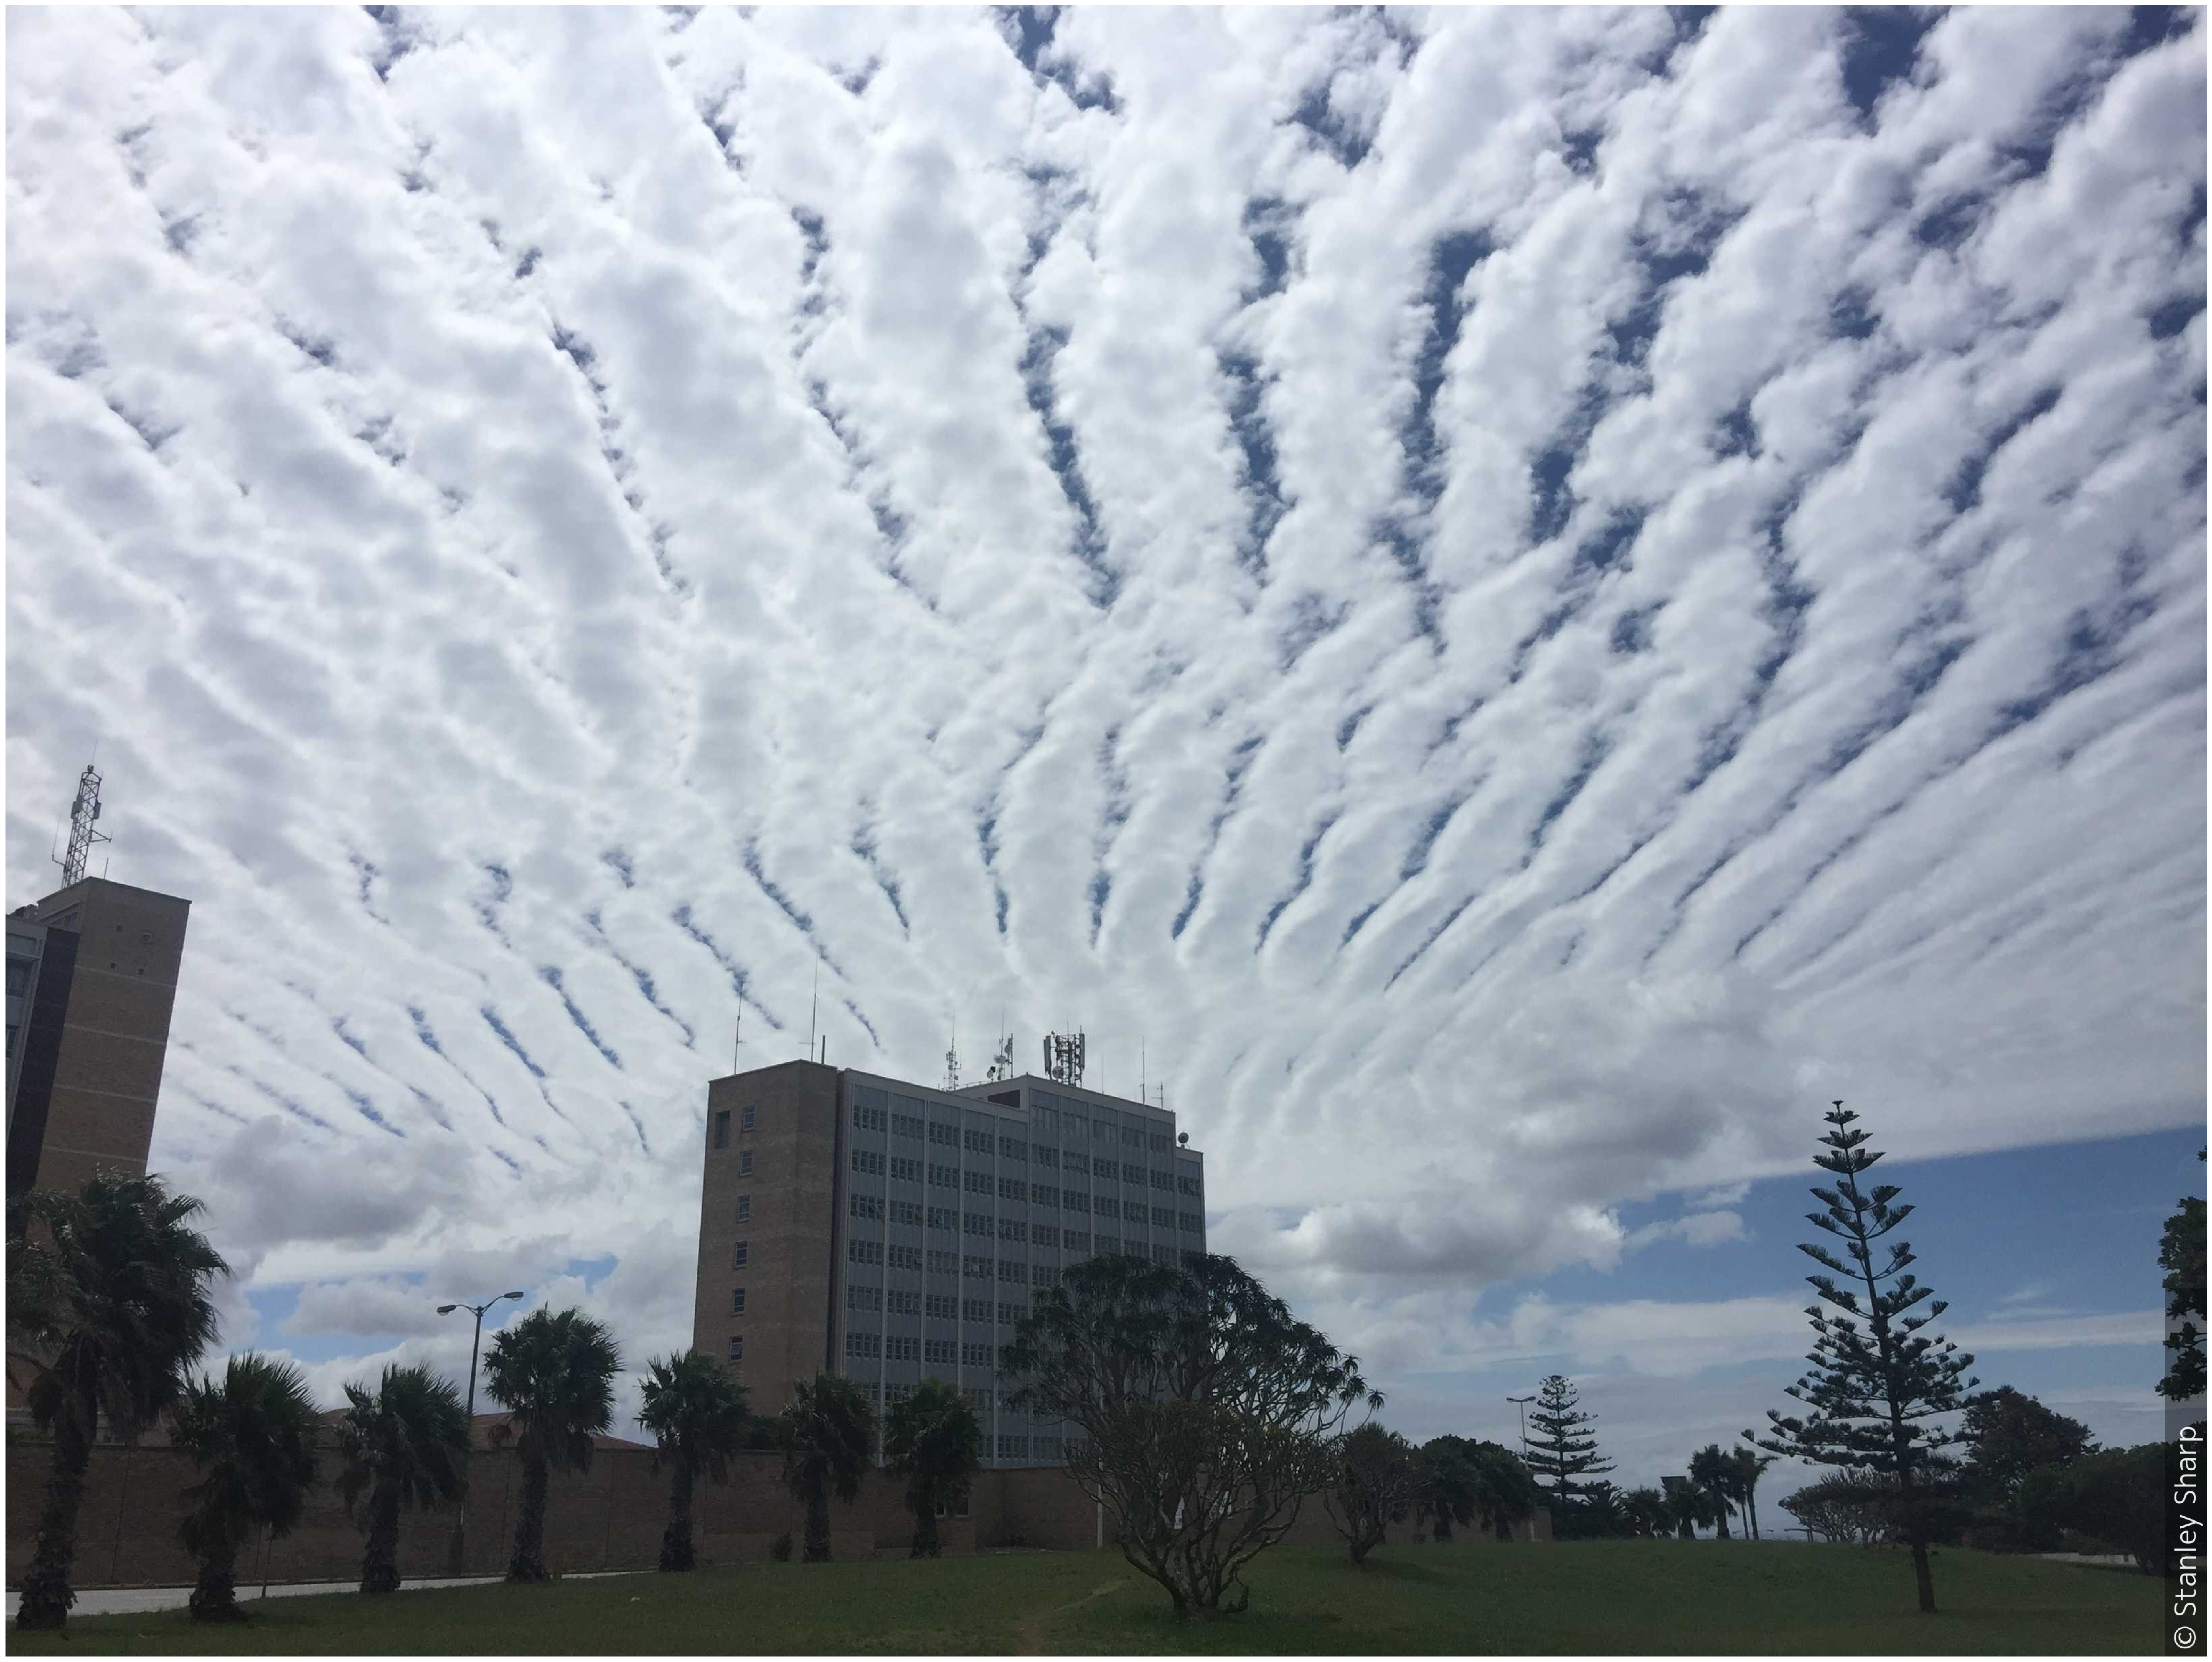
\includegraphics[width=0.6\linewidth,keepaspectratio]{CloudAtlas_CM5.eps}
        \caption{CM=5の中層雲(International Cloud Atlasより引用)}\label{CloudAtlas}
        \end{figure}
     この中層雲がどのような地域にできるのか、そのメカニズムとともに説明しなさい。また、図\ref{Sate}において、どのあたりにこの中層雲があるかを示しなさい。
        \begin{figure}[h]
        \centering
        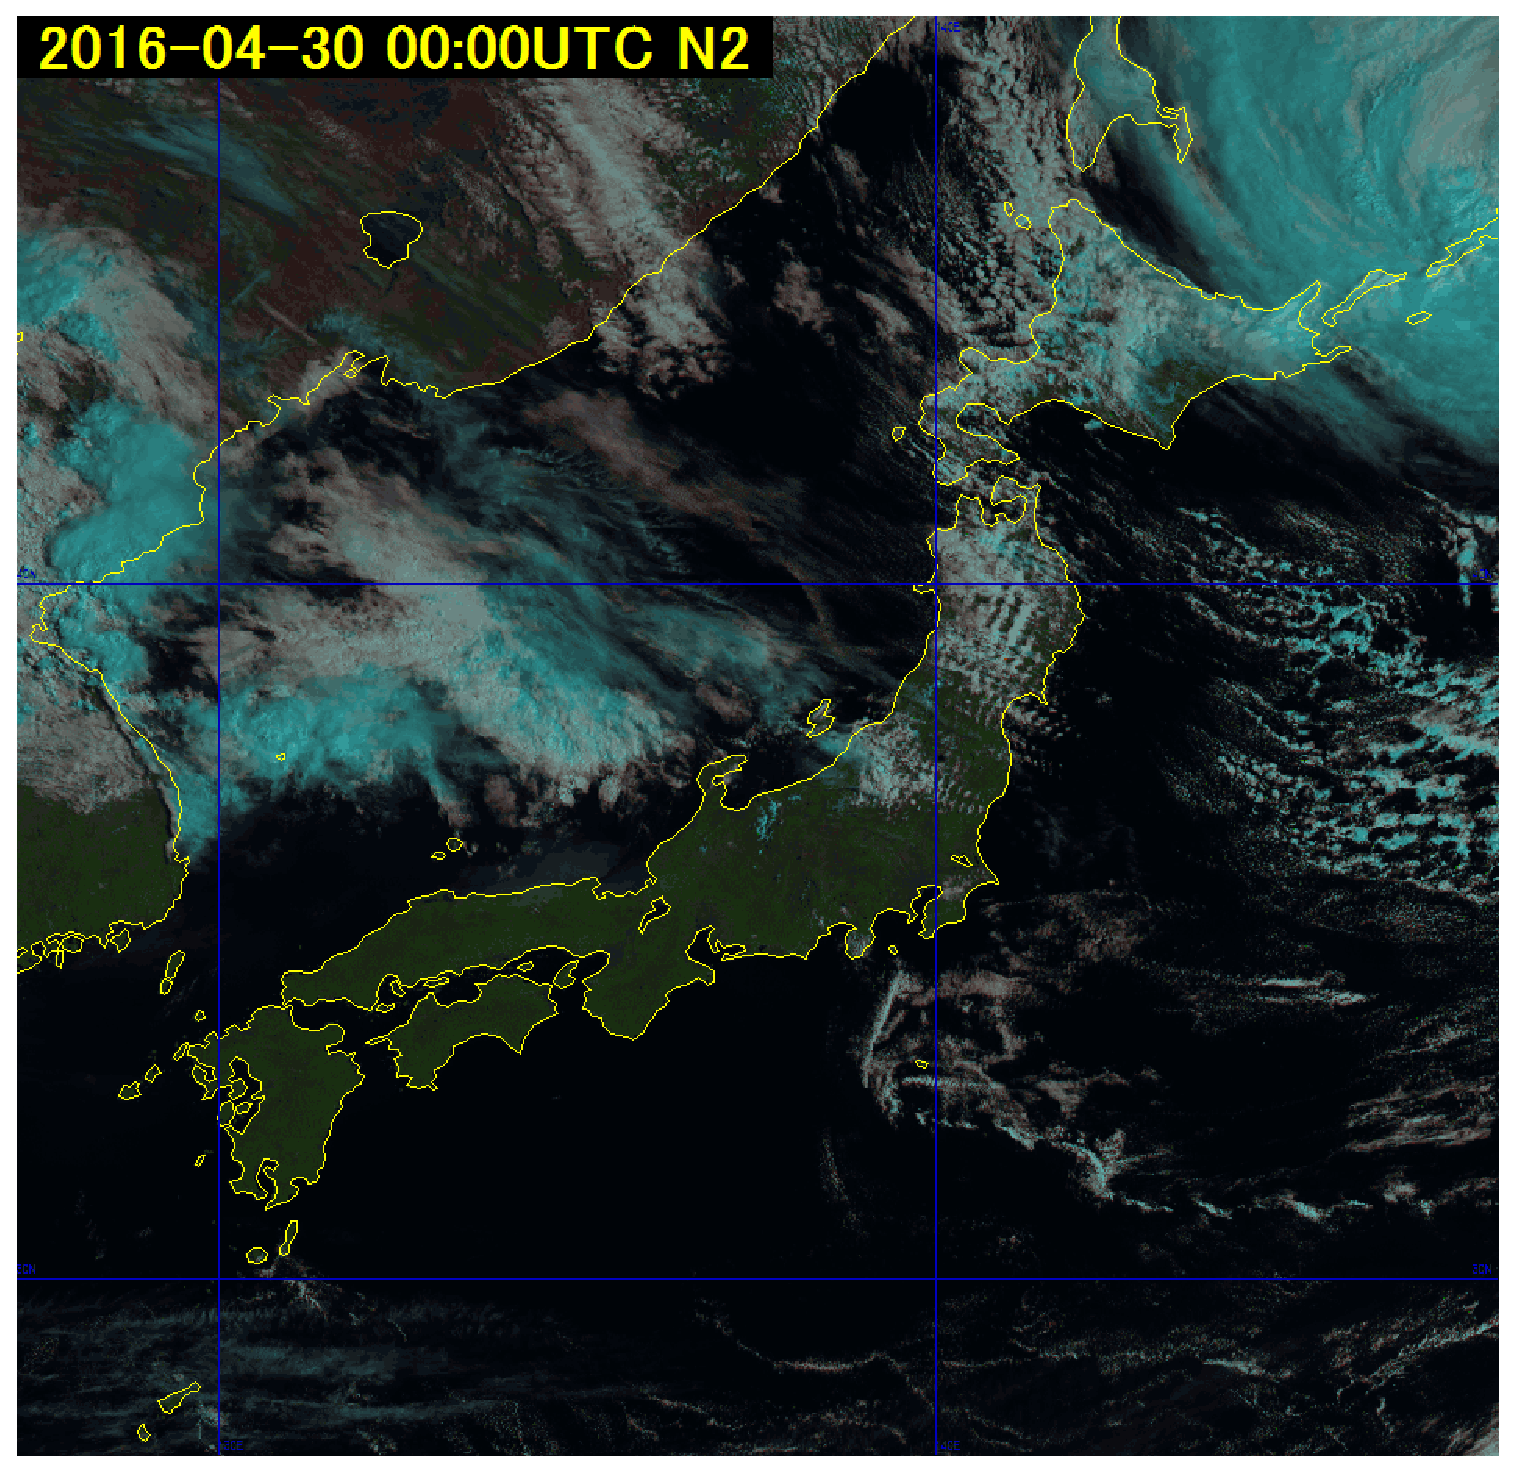
\includegraphics[width=0.6\linewidth,keepaspectratio]{Sate.eps}
        \caption{2016/4/30 午前9時の国内衛星画像(気象衛星センターサイトより引用)}\label{Sate}
        \end{figure}

    \item 晴天の夜間、風が弱く地表面の放射冷却が強い時、周囲を山や尾根で囲まれた盆地や谷間に冷やされた空気が湖のように溜まる現象として「冷気湖(cold air lake)」が知られている。この現象のメカニズムを今回学んだことを元に説明しなさい。

\end{problems}

\section{答案}
\begin{problems}
% 以下に解答を作成してGit Push。
\item 

\item 

\item 

\end{problems}

\section{読書案内}
メソ気象学は境界層気象学や大気熱力学と関わる分野でもあり、そちらで紹介した読書案内が参考になる。
それ以外のメソ特有の書籍として、以下を紹介する。

\begin{itemize}
\item 小倉義光 1997 "メソ気象の基礎理論" 東大出版
\item 大野久雄 2001 "雷雨とメソ気象" 東京堂出版
\item 吉崎正憲,加藤輝之 2007 "豪雨・豪雪の気象学" 朝倉書店
\item 加藤輝之 "図解説中小規模気象学" \url{https://www.jma.go.jp/jma/kishou/know/expert/pdf/textbook_meso_v2.1.pdf}
\item R.A.Houze 2014 "Cloud Dynamics" Academic Press
\item R.A.Pielke 2013 "Mesoscale Meteorological Modeling" Academic Press
\end{itemize}


\end{document}

